\documentclass{article}

\usepackage[utf8]{inputenc} %character coding
\usepackage[english]{babel} %language formating
\usepackage{amsfonts} % some math fonts
\usepackage{amsmath, amsthm, amssymb} %some more math packages
\usepackage{graphicx} % for plots ...
\usepackage{booktabs} %% for nice tables
\usepackage{caption} %% for float captions

\usepackage{hyperref} %% inportant for references. Can work without, but better to have it.


\newcommand{\hydjet}{HYDJET++ } %% this is how you define new command


\title{A Small \LaTeX{} Article Template\thanks{To your mother}}
\author{Your Name  \\
	Your Company / University  \\
	% \and 
	% The Other Dude \\
	% His Company / University \\
	}

\date{\today}
% Hint: \title{what ever}, \author{who care} and \date{when ever} could stand
% before or after the \begin{document} command
% BUT the \maketitle command MUST come AFTER the \begin{document} command!

%% HERE BEGIND DOCUMENT
\begin{document}

\maketitle


\begin{abstract}
Short introduction to subject of the paper \ldots
\end{abstract}

\section{Introduction}
Make it possible for all to write documents with \LaTeX{}!

\paragraph{Outline}
First we start with a little example of the article class, which is an
important documentclass. But there would be other documentclasses like
book \ref{book}, report \ref{report} and letter \ref{letter} which are
described in Section \ref{documentclasses}. Finally, Section
\ref{conclusions} gives the conclusions.



\section{Documentclasses} \label{documentclasses}

%% this is how you make bullet list
\begin{itemize}
\item article
\item book
\item report
\item letter
\end{itemize}

%% this is how you make numbered lists
\begin{enumerate}
\item article
\item book
\item report
\item letter
\end{enumerate}

%% another type of lists
\begin{description}
\item[article\label{article}]{Article is \ldots}
\item[book\label{book}]{The book class \ldots}
\item[report\label{report}]{Report gives you \ldots}
\item[letter\label{letter}]{If you want to write a letter.}
\end{description}


%% suppress section number by *
\section*{Some useful tips}
\label{tips}
Some utilities require multiple compilation, e.~g. references such as are in this example need the code to be compiles $\times 2$.
% dollars do simple math

$$ a = b+c $$


Here is an example of nice \textbf{equation}, see Eq. \ref{equation}.
\begin{equation}
 a = b+c
 \label{equation}
\end{equation}

You can also find an example of how to add figures in Fig. \ref{fig} and tables in Tab. \ref{tab:particles_hydjet}. In documentation, these are called floats.
\begin{figure}[h]
  \begin{center}
      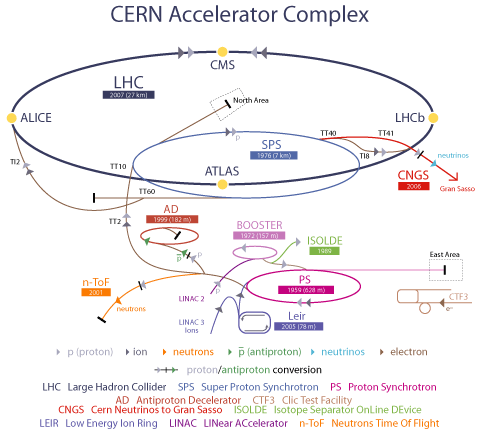
\includegraphics[width = 0.6 \textwidth]{img/cern}
      \caption{CERN accelerator complex.}
    \label{fig}
  \end{center}
\end{figure}

\begin{table}[h]
  \begin{center}
  \begin{tabular}{l c c c l}
  \toprule
				& particles	& mass [GeV/$c^2$]	& quark content 	& {\tt Abs(pdg1)} \\
    \midrule
%         $p, \bar{p}$		& 			&   \\
%         $\pi^{\pm}$		& 			&   \\
%         $K^{\pm}$		& 			& \\
        charged			& $(p+\bar{p})$ & $ 938.272046 \pm 0.000021 $	& $(uud)$	& 2212 \\
				& $\pi^{\pm}$   & $139.57018 \pm 0.00035 $	& $(u\bar{d})$	& 211 \\
				& $K^{\pm}$ 	& $493.677 \pm 0.016$	& $(u\bar{s})$	& 321 \\
        $\Lambda, \bar{\Lambda}$ & $\Lambda^0 + \overline{\Lambda^0}$ &	$1115.683 \pm 0.006  $	& $(sud)$	& 3122 \\
% 				& $\Sigma^+ + \overline{\Sigma^+}$     & 3222 \\
% 				& $\Sigma^- + \overline{\Sigma^-}$     & 3112 \\
				& $\Sigma^0 + \overline{\Sigma^0}$ & $ 1192.642 \pm 0.024$	& $(sud)$     & 3212 \\


  \bottomrule

  \end{tabular}
  \caption{Particle states used for charged and lambda distributions. The states are uniquely identified in \hydjet via {\tt pdg1} flag. Displayed content for either baryon or positive meson  only.}
  \label{tab:particles_hydjet}
  \end{center}
\end{table}


Wast documentation is available online, do not worry when you find multiple solutins to your problems. In \LaTeX, there is usually more than one way to do things, \cite{numberref}.






\section{Conclusions}\label{conclusions}
There is no longer \LaTeX{} example which was written by \cite{doe}.


\begin{thebibliography}{9}
\bibitem[Doe]{doe} \emph{First and last \LaTeX{} example.},
John Doe 50 B.C.
\bibitem{numberref} Normal numbered reference.
\end{thebibliography}

\end{document}
